% Experimente as seguintes opções das classes-padrão (article, report e book):
% - twocolumn
% - landscape
% - a4paper
% - leqno
% - fleqn
% - notitlepage
% - draft
\documentclass[a4paper,12pt]{report}
	\usepackage[ansinew]{inputenc}
	%\usepackage{fourier}
	\usepackage{ae}	
	\usepackage[brazil]{babel}
	\usepackage{xcolor}
	\usepackage{graphicx}
	%\usepackage{indentfirst}
	\usepackage{psfrag}
	\usepackage{booktabs}
	\usepackage{usandoLaTeX}
		
	\graphicspath{{./figuras/}}
			
	% O comando \date altera o texto-padrão da data.
	%\date{Sexta-feira\dots\ dia de happy-hour} % EXPERIÊNCIA: descomente esta linha.			
	
	\markright{Cabeçalho da página}  % Utilize o pacote fancyhdr (fancy header) para
	\pagestyle{myheadings}           % um controle muito melhor do cabeçalho e rodapé.
	
	%\pagenumbering{roman} % Experimente trocar o argumento para "arabic" ou "Roman"
	
	\hyphenation{lem-bre-se}
	
	
	\title{{\Huge\bfseries O título do meu trabalho}} % Use sempre {} para delimitar a ação de seus comandos...
	                                                  % Não confie nas chaves do comando \title, por exemplo.
	                                                  % Internamente, pode ocorrer de eles serem removidos.
	
	\author{%
		I. R. Pagnossin\thanks{eu@mesmo.com} \\ Universidade de São Paulo
		\and
		Segundo autor\thanks{meu@colega.com} \\ Outra instituição}
		
\begin{document}

	% Este comando imprime os dados da capa (título do trabalho, autor e data)	
	\maketitle % EXPERIÊNCIA: comente esta linha.

	%-------------------------------------------------------------------------	
	\begin{abstract}
		Para escrever um resumo (ou \foreign{abstract}) do trabalho, utilizamos
		o ambiente \env{abstract}. A formatação é totalmente gerenciada pelo \LaTeX,
		restando ao autor apenas preocupar-se com o conteúdo.
		
		Note também a ação do pacote \pkg{babel}: sem ele, ao invés de ``resumo'',
		teríamos ``\foreign{abstract}''. Experimente!
	\end{abstract}

	%-------------------------------------------------------------------------
	\tableofcontents % O sumário, criado automaticamente pelo LaTeX a partir
	                 % dos comandos \chapter, \section, etc.

	Este texto provavelmente está no lugar errado, pois não tem uma seção ou
	capítulo associado. Como está, ele pertence ao sumário (ToC, \foreign{table
	of contents}).
	
	%-------------------------------------------------------------------------
	\listoffigures   % A lista de figuras, criada automaticamente pelo LaTeX
	                 % a partir dos ambientes "figure."

	Este texto provavelmente está no lugar errado, pois não tem uma seção ou
	capítulo associado. Como está, ele pertence à lista de figuras (LoF,
	\foreign{list of figures}).
	
	%-------------------------------------------------------------------------
	\listoftables    % A lista de tabelas, criada automaticamente pelo LaTeX
	                 % a partir dos ambientes "table"

	Este texto provavelmente está no lugar errado, pois não tem uma seção ou
	capítulo associado. Como está, ele pertence à lista de tabelas (LoT,
	\foreign{list of tables}).

	%-------------------------------------------------------------------------	
	\chapter{Conceitos e métodos}\label{ch:conceitos}
	
	Observe que o comando \cs{chapter} não define apenas a forma como o título
	é exibido. Ele permite também a utilização do comando \cs{label}, para
	referências cruzadas, e inclui o título no sumário (ou no bookmarks, no caso
	de um documento PDF).
	
	% Aqui eu inicio uma seção do trabalho e atribuo-lhe um rótulo (sec:QHE), que
	% poderá ser utilizado pelo comando \ref em qualquer lugar do documento.
	%-------------------------------------------------------------------------
	\section{Esta é uma seção}\label{sec:secao}
		
	O \LaTeX\ não endenta o primeiro parágrafo de uma seção (ou subseção, etc.).
	Se você quiser que isto ocorra, apenas importe o pacote \pkg{indentfirst} (o
	comando \cs{indent} não funciona aqui).
	
	%-------------------------------------------------------------------------
	\subsection{Esta é uma subseção}\label{sec:subsecao}
	
	%\setlength{\mathindent}{2cm} % EXPERIÊNCIA: acrescente a opção "fleqn" no \documentclass{} e descomente esta linha.
		
	O comportamento padrão do \LaTeX\ no que concerne as expressões matemáticas
	que têm sua própria linha (modo de exibição \emph{display style}) é centralizá-% O que acontece se você tirar este comentário?
	las. E a numeração, se houver, é alinhada à margem direita da página. Por
	exemplo,
	\begin{equation}\label{eq:QHE}
		R_H = \frac{R_K}{N}
	\end{equation}
	é a expressão do efeito Hall quântico inteiro. $R_H$ é a resistência Hall, $R_K$
	é a constante de Von-Klitzing e $N = 1, 2, \ldots$

	Mas você tem duas alternativas, dadas pelas opções \opt{leqno} e \opt{fleqn}.
	Elas colocam a numeração e a expressão à esquerda, respectivamente. A numeração
	é alinhada com a margem esquerda e a expressão, sofre endentação dada pelo
	comprimento \cs{mathindent}, que pode ser alterado. Mas atenção: este	comprimento
	só estará definido quando a opção \opt{fleqn} estiver em voga.
	
	\begin{figure}
		\centering
		\psfrag{A}[l][l]{\parbox{0.25\textwidth}{\tiny\color{red}Este texto só aparece se
			você gerou um documento PostScript. Neste caso este é um texto que utiliza a mesma
			fonte do corpo do documento.}}
		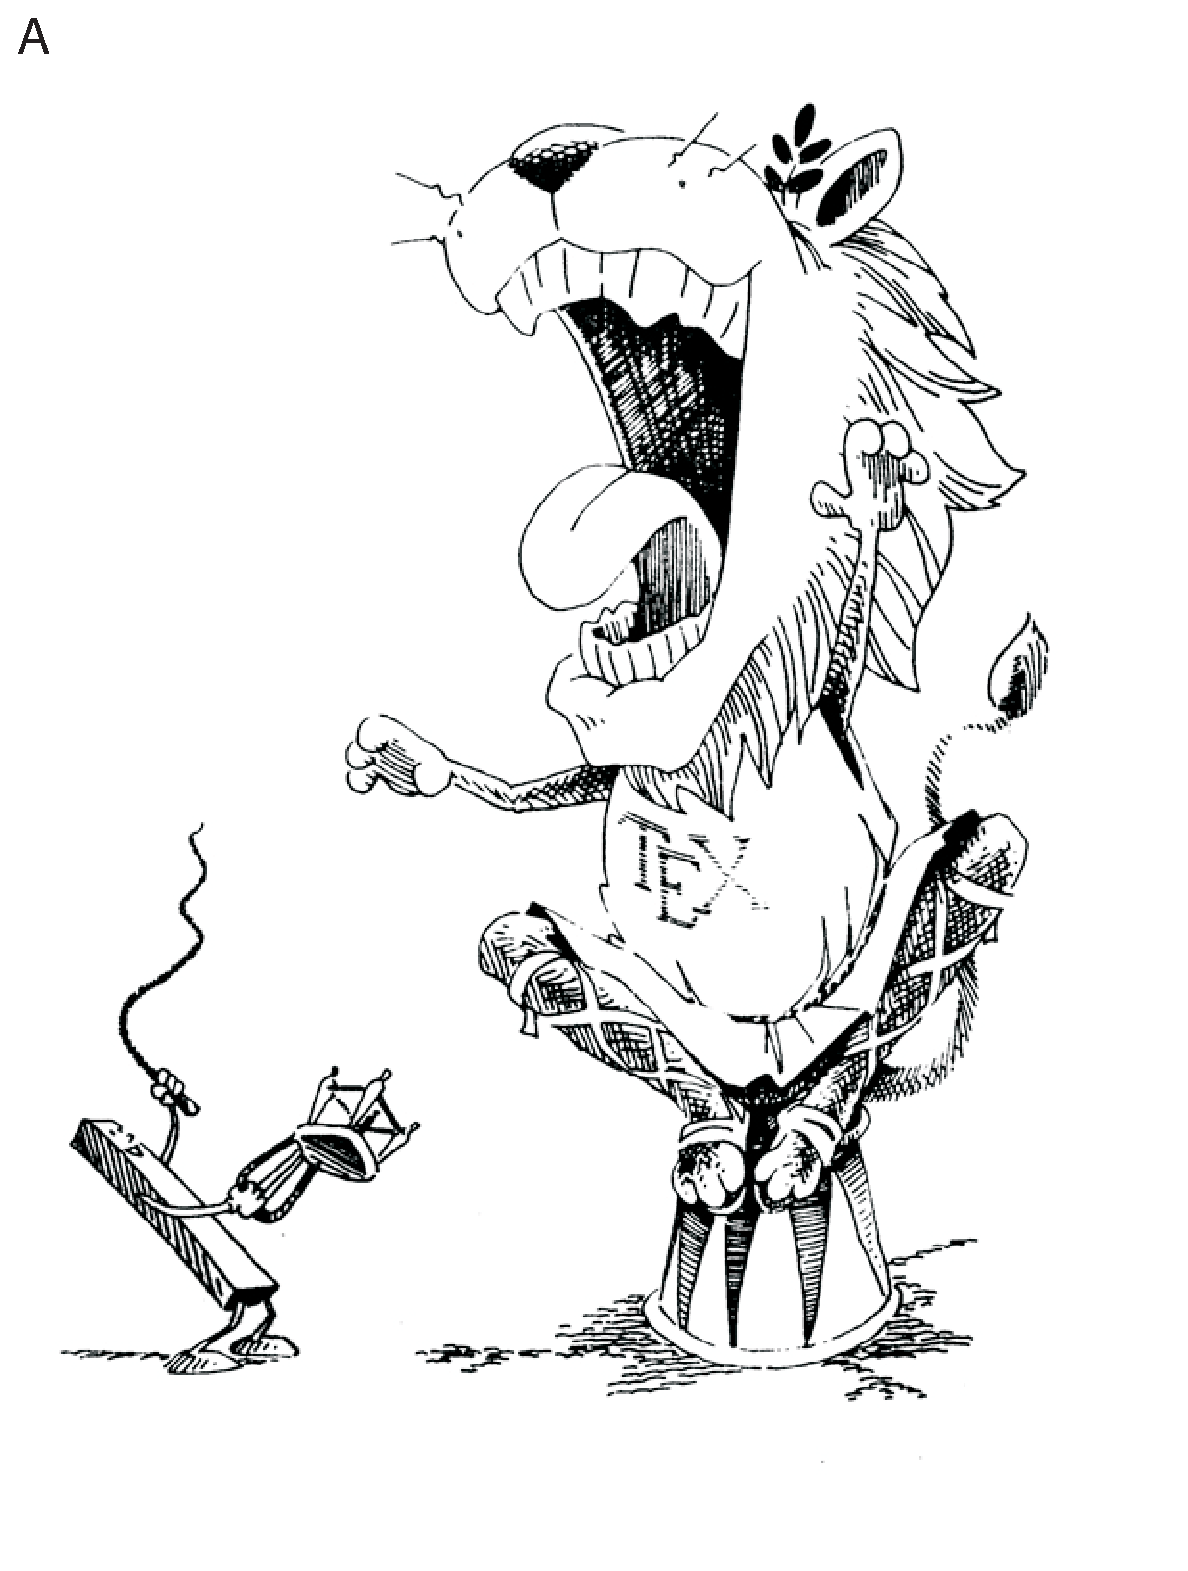
\includegraphics[width=0.4\textwidth]{Controlling_TeX}
		\caption{ilustração do capítulo ``controlling \TeX'' do livro \cite{knuth}.}
		\label{fig:TeX}
	\end{figure}

	\begin{table}
		\centering
		\begin{tabular}{ccc}
			\toprule
			1 & 2 & 3 \\
			\midrule
			4 & 5 & 6 \\
			\bottomrule
		\end{tabular}
		\caption{legenda de uma tabela qualquer.}
		\label{tab:tabela}
	\end{table}

	%-------------------------------------------------------------------------
	\section*{Uma seção sem número e que não aparece no sumário}
		
	A versão com asterisco do comando \cs{section} inibe tanto a numeração como
	a presença da seção no sumário. Tipicamente, isto é utilizado em seções de
	menor hierarquia (\cs{subsubsection} na classe \cls{article}, por exemplo).	
	
	%-------------------------------------------------------------------------
	\subsubsection*{Por alguma razão não nos interessa colocar todo este
	título no sumário}
		
	Ao iniciar uma seção, às vezes pode ser necessário inserir um nome alternativo
	no sumário. Isto ocorre, por exemplo, quando o título da seção é demasiadamente
	grande, como aqui. Neste caso, passamos o nome alternativo ao comando
	\cs{section} na forma de um argumento opcional, isto é, entre colchetes.
	
	\paragraph{\S1\textordmasculine}
	
	Observe que o texto imediatamente após o comando \cs{paragraph} faz parte do
	parágrafo iniciado por \cs{paragraph}, ainda que haja uma linha em branco ou
	um comando \cs{par} entre eles.
	
	\subparagraph{\P} Idem para \cs{subparagraph}, mas atenção ao espaço vertical
	inerente a estes comandos.
	
	%-------------------------------------------------------------------------
	\appendix
	\chapter{A declaração \cs{appendix}}\label{ap:rotulo}
	
	A declaração \cs{appendix} informa ao \LaTeX\ que as seções \emph{iniciadas}
	a	partir dali são apêndices do trabalho.
	
	Aqui acontece algo curioso: observe que a compilação deste documento gera
	duas mensagens de aviso:

	\newlength\mylength
	\settowidth\mylength{\ttfamily LaTeX Font Warning: Font shape OMS/cmtt/bx/n undefined}

	\begin{center}
		\begin{minipage}{\mylength}
			\ttfamily
			\begin{tabbing}
				LaTeX Font Warning: \=Font shape OMS/cmtt/m/n undefined\\
				                    \>using OMS/cmsy/m/n
			\end{tabbing}
		\end{minipage}
	\end{center}
	
	% obs.: o comando \fntattr foi definido em defs.sty e defs.tex
	Isto ocorre porque o caráter \textbackslash\ no título da seção não está
	definido no \foreign{encoding} OMS, família \fntattr{cmtt} (computer modern
	typewriter), série \fntattr{m} (média) e forma \fntattr{n} (normal ou para
	cima). O compilador, então, decidiu utilizar o caráter de família cmsy
	(computer	modern symbol),	com a mesma série e forma.
	
	Neste caso, você pode resolver este problema importando o pacote
	\pkg{fontenc}	com a opção (\foreign{encoding}) \fntattr{T1}, ou ainda melhor,
	o pacote \pkg{ae}. Faça isso e observe como a mensagem some. Aliás, o
	\foreign{bad box} também é resolvido com isso, pois o que o estava gerando
	era a palavra ``matemática'' na seção~\ref{sec:subsecao}: uma palavra
	acentuada que, na codificação-padrão (\fntattr{OT1}), o \LaTeX\ não sabia
	como separar as sílabas.
	
	\begin{quotation}
		\noindent\obs você não precisa conhecer estes códigos, apenas
		lembre-se de um caráter qualquer que você queira pode não estar definido
		para a fonte em uso.

		\noindent\obs a segunda mensagem de erro é apenas uma afirmação da
		primeira.
		
		\noindent\obs você percebeu que o texto \textbf{obs.} no início deste
		parágrafo é gerado por um comando definido no pacote \pkg{usandoLaTeX},
		e que ele utiliza um contador para gerenciar a numeração das observações?
	\end{quotation}	
	
	%-------------------------------------------------------------------------
	\chapter{O ambiente \env{appendix}}
	
	Alternativamente à declaração \cs{appendix}, você pode colocar as seções que
	compõem os apêndices dentro do ambiente \env{appendix}.\footnote{Para inserir
	uma nota de rodapé, simplesmente utilize o comando \cs{footnote}.}

	%-------------------------------------------------------------------------
	\begin{thebibliography}{+}
	\bibitem{knuth} D. E. Knuth, \textsl{The \TeX book}, Addison-Wesley, 1991.
	\end{thebibliography}

\end{document}